\documentclass{article}
\usepackage{graphicx}
\usepackage[backend=biber,style=ieee]{biblatex}
\usepackage[a4paper,margin=2.5cm]{geometry} 
\usepackage{xcolor}
\usepackage{gensymb} % For \degree
\usepackage{bm}
\usepackage{tabularx}
\usepackage{parskip}
\usepackage{float}
\usepackage{tikz}
\usepackage{placeins}
\usepackage{amsmath}
\usepackage{makecell}
\usepackage{comment}
\usepackage{tikz}
\usepackage{multirow}
\usepackage{booktabs}
\usetikzlibrary{positioning} % Required for 'below=of' syntax
\usetikzlibrary{shapes.geometric} % Required for the 'diamond' shape
\usetikzlibrary{positioning,fit,arrows.meta}
\addbibresource{./bib/references.bib}




\newcommand{\todo}[1]{\textcolor{red}{\textbf{TODO:} #1}}
\newcommand{\fixme}[1]{\textcolor{orange}{\textbf{FIXME:} #1}}
\newcommand{\words}[1]{\textcolor{blue}{\textbf{WORDS:} #1}}

\usepackage[hidelinks]{hyperref}


\graphicspath{{figures/}}


\begin{document}

\input{sections/FrontPages/titlepage}

\input{sections/FrontPages/abstract}

\addcontentsline{toc}{section}{Acknowledgements}
\section*{Acknowledgements}
I would like to express my sincere gratitude to Professor Zhiqiang Zhang for his continuous 
support and guidance throughout this project. Professor Zhang's insights and advice during 
this project, in particular the explanation of Lie group theory and in-depth explanation of filters, 
were invaluable in shaping the direction of my work. In addition, offering his personal
copy of Body Sensor Networks to aid in my understanding was highly appreciated.

I would also like to acknowledge the authors and maintainers of the publicly available
datasets of BROAD. Their efforts in collecting and labelling high-quality
IMU data and optical motion capture ground truth enabled the training, testing, and 
validation of the neural network. I am grateful for their contributions and cite them
accordingly in this report.  


\newpage

\tableofcontents

\input{sections/FrontPages/LoF}

\input{sections/FrontPages/LoT}



\input{sections/Intro/introduction}

\newpage
\section{Societal Factors}

\subsection{Healthcare \& Rehabilitation}
In healthcare and rehabilitation, there is a wide need for orientation estimation from limb kinematics to assessment protocols for 
Axial Spondyloarthritis \fixme{add cites}. However, these studies
also highlight orientation drift due to IMUs as a limitation to their uses. 


Franco et al, highlights that IMUs have not widely been used for orientation estimation in a clincal setting due to gyroscopic drift \fixme{cite}.
Specifically, the study conducted range of motion tests that uses an IMU and Kalman Filter under constrained movements. The BASMI
movements performed and recorded all spanned for approximately 30s and achieved and RMSE = 2.0 degrees for joint flexion. 
However, all of these trials were performed
in a controlled laborartory setting with constrained movements to limit the accumulation of drift. Further, this
sensor alignment assumes that the sensors reflect the actual tilt of the
spine in the sagittal and frontal planes, and that the spine axial rotation is zero at t0 \fixme{cite}.
Under these constraints and assumptions, trying to extend this protocol outside of the laborartory and into clinical settings which have a lot 
of magnetic disturbances or under continuous monitoring of uncontrolled motions, their approach breaks down and drift accumulates. The proposed solution
in \fixme{section} serves as a way of extending and enabling further investigation of range of motion under non-constrained and continuous monitoring.
However, it is important to acknowledge that this proposed solution is based on data found in \fixme{section} compared to spinal kinematics data. However,
the dataset does include slow small rotations which is representative of the types of motions that Franco et al performed.  


\subsection{Agriculture}
\subsection{}

\begin{comment}
    Sy et al \fixme{cite} highlight that IMUs suffer from global drift 
and that these can be corrected with other sensors such as camera-based solutions but also mention the extra need of people needing to carry these 
cameras or that it requires setup \fixme{cite}. Wittmann et al also highlights the need for a homogenous magnetic field to correct gyroscope
drift \fixme{cite}. 
\end{comment}



\newpage
\section{IMU Basics and Operational Principles}


\input{sections/IMU_background/gyro}

\input{sections/IMU_background/accel}

\subsection{Magnetometer: Operations and Errors}
Magnetometers measure the local magnetic field along its orthogonal axes $m^x,m^y,m^z$. 
The magnetometer can be used to determine the 
heading (yaw) of an object. Sensor fusion/filtering algorithms are dependent on sensing the local
magnetic field to eliminate drift in the azimuth (yaw) portion of orientation estimates \cite{bachmann_2004_an}.
It does this by assuming that the measured local field vector provides a reference 
relative to Earth's field. However, changes in the local field due to other field sources, can 
distort this measurement which gives rise to erroneous heading corrections. 

\subsubsection{Magnetometer Error Sources and Effects}
\label{sec:magerrors}
\subsubsection*{Hard-Iron/ Soft-Iron}
Hard-iron is a constant additive magnetic field applied to the sensor 
due to the interaction of magnetic fields  \cite{luiz_2011_geometric}. 
This interaction between these sources leads to a constant vector being applied to the measurement.


Soft-iron effects are generated by the interaction of an external magnetic field on any 
ferromagnetic materials near the sensor \cite{luiz_2011_geometric}. The resulting magnetic field depends
on the magnetic field vector with respect to the orientation of the soft iron material \cite{a2026_calibration}. 




\newpage
\section{Dataset (BROAD)}


Testing some stuff

\newpage
\section{Manifold Unscented Kalman Filter}

\subsection{Kalman Filter Overview}
The Kalman filter (KF) is an optimal recursive estimator used to estimate a 
state under noisy measurements and uncertain dynamics. It works under an assumption that the relationship
between our state and measurements can be modelled as linear and Gaussian \fixme{cite intro to KF}.

\begin{table}[!htbp]
\centering
\small
\begin{tabular}{p{3.5cm} p{8.5cm}}
\hline
\textbf{Term} & \textbf{Description} \\
\hline
State Vector ($\mathbf{x}$) & The quantity the filter is trying to estimate. \\
State Estimate Covariance ($\mathbf{P}$) & The uncertainty the filter has in its state estimation. \\
Process Noise Covariance ($\mathbf{Q}$) & The uncertainty the filter has in its process model, i.e. how much the filter trusts the dynamics used to propagate the state. \\
Measurement Noise Covariance ($\mathbf{R}$) & The uncertainty the filter has in its measurement values, used to correct the state. \\
Kalman Gain ($\mathbf{K}$) & Balances the weight given to the process model prediction versus the incoming measurement. \\
\hline
\end{tabular}
\caption{Kalman Filter Terms and Definitions}
\label{tab:kf_terms}
\end{table}

The filter implements a two step process of prediction and update. The predicition
propagates our state estimation and the update corrects the state estimation using one
or multiple measurements. The covariance P is updated by the K after every new sensor value to reflect
the new information the filter has gained about the system.

However, the KF breaks down for orientation estimation due to some key factors. First, quaternion kinematics are
non-linear (\fixme{see SO(3) equation}) and the assumption that the relationship is linear is violated. Second, as the relationship is non-linear, this
breaks the Gaussian noise process model as propagation through a non-linear function produces a non-Gaussian output. Third,
as quaternions exist in SO(3) and not Euclidean space, adding a Gaussian term to the state can push it off the manifold.




\subsection{Unscented Kalman Filter}
The Unscented Kalman Filter (UKF) is an extension of the KF that allows for non-linear relationships to be more accurately modelled by the filter. 
Traditionally, to apply a KF to a non-linear relationship an extended KF (EKF) is used which linearises all non-linear 
models through the use of Jacobian matrices that are evaluated at the current state estimate. \fixme{cite Julier}. 
However, better performance tends to be achieved by a UKF for orientation estimation as a UKF gives more accurate covariance propagation at 
larger rotations \cite{kraft_2003_a} \fixme{cite Julier}.

Sigma points are drawn from a specific, deterministic algorithm that when a non-linear function is applied to these points; a set of $2n + 1$ transformed
points are left ($n = 3$ for a 3D error state, giving $7$ sigma points).
These sigma points are then used to reconstruct the mean by taking a weighted average of these points and the weighted outer product
for the covariance. 

However, with the non-linear propagation addressed, computing a weighted mean of quaternions directly is geometrically invalid. This is due to
quaternions exisiting on the SO(3) manifold, as the element-wise average of quaternions does not lie on the unit sphere and therefore does not represent a valid rotation.  

For an in-depth derivation regarding the UKF see \fixme{cite Julier}.

\subsection{The Manifold Problem}
The core issue of the UKF is that it assumes that the x lies within Euclidean space, however quaternions lie on the SO(3) manifold. So computing the mean
and adding the measurement noise to the state is geometrically invalid, thus the state that is estimated is also invalid.

The solution to this problem is to perform any arithmetic computations that the UKF requires within the local tangent space (so(3)). By taking the current 
state estimate (quaternion on the SO(3) manifold) and mapping it to and from Euclidean vector space, the predict and update steps are performed validly 
and the geometric representation of the state is conserved. Brossard et al and Crassidis et al
explore and show this within their UKF-Manifold and Unscented Quaternion Estimator (USQUE) implementations \fixme{cite UKF-M and USQUE}.

Thus the implementation used in this project is based on UKF-M as it is generalisable to various manifolds not just SO(3).

\subsection{Filter Design}



\subsection{Filter Setup}

Table 1 below shows the configuration used for the UKF for each of the scenarios. 

\label{sec:filtersetup}
\begin{table}[!htbp]
\centering
\small
\begin{tabular}{p{2.0cm} p{5.0cm} p{5.0cm} p{1.5cm}}
\hline
\textbf{State} & \textbf{Process Noise ($Q$)} & \textbf{Measurement Noise ($R$)} & \textbf{Sampling Rate} \\
\hline
\makecell[l]{$q_w, q_x, q_y, q_z,$ \\ $\omega_{b,x}, \omega_{b,y}, \omega_{b,z}$}
&
Gaussian noise determined by rest phases
&
Gaussian noise determined by rest phases
&
$286\,\text{Hz}$ \\
\hline
\end{tabular}
\caption{UKF configuration}
\label{tab:filtersetup}
\end{table}

The state estimates the orientation that is determined by integrating gyroscope measurements
where there is an assumed slowly varying additive bias applied to the gyroscope. The matrix $Q$ handles the uncertainty
the filter has in the process model (gyro integration). The measurement model assumes that accelerometer updates
are the measured specific force that aligns with gravity (low linear acceleration), and the magnetometer is a reference
of the local Earth's field. The matrix $R$ is the uncertainty that the filter has in accelerometer and magnetometer
updates and is adaptively weighted.   

\subsubsection{Adaptive Gating for Disturbed Measurements}

The matrix $R$ applied an adaptive scheme where disturbed accelerometer and 
magnetometer measurements were downweighted for correcting the orientation. The initial covariance
was determined by taking a mean of all measurements for each sensor during the rest periods, 
and subtracting this mean, to get residuals from the sensors. These
residuals were then computed as the covariance which is modelled as Gaussian noise and before each correction applied by the filter, 
a heuristic approach was taken by tuning arbitrary tolerances to accept or downweight the sensor
measurements. If measurements were deemed unreliable, then the matrix $R$ would be multiplied by a scalar
value to downweight updates during corrections, this scheme was selected because outright rejection of measurements caused 
discontinuous orientation estimates.

The matrix $Q$, also took a similar approach where gyro bias was determined through subtracting 
the mean during rest phases and these residuals were computed as the covariance which was modelled to be Gaussian noise. 
\newpage




\newpage
\section{Deep Learning Architecture}

\begin{itemize}
  \item TCN Design so causal conv, conv1d, activation functions etc.
  \item Learning - Loss Functions, Explain problem of overfitting and why we need regularisation, optimisers (explain gradient descent), learning rate
\end{itemize}

\subsection{Aims of the Deep Learning Model}
Referring back to \hyperref[sec:problem]{section 1.2}, the overall problem 
is to implement a model that can output gyroscopic corrections 
$\Delta\boldsymbol{\omega}_t = [\Delta\omega_x,\Delta\omega_y,\Delta\omega_z]^\top$
that when subtracted from our measured angular rate, and fused with other
sensors such as an accelerometer and magnetometer leads to an orientation 
estimate, that is more accurate to the ground truth orientation of an 
object compared with only sensor fusion. 

The motivation for learning $\Delta\boldsymbol{\omega}_t$ 
comes from the fact that while sensor fusion techniques of downweighting 
or skipping of the accelerometer and magnetometer when they are unreliable
, drift cannot be mitigated due to the accumulation of gyroscopic bias 
and noise \fixme{cite, cite2}. 

\subsection{Model Selection}
\subsubsection{Recurrent Neural Networks (RNNs)}
The first type of model that was considered is a RNN. RNNs stem from an 
idea of recurrence, that is that the output depends on some input at time
t and an internal state of the model that holds information about previous
outputs of the model. The general idea can be described by the equation

\begin{equation}
\hat{y} = f_{model}(x_t, h_{t-1})
\end{equation}

where $\hat{y}$ is the output, $f_{model}$, is a function that describes the model,
$x_t$ is the input at time t, and $h_{t-1}$ is a vector state that
describes the internal state of the model at the previous time step. Expanding
on this the state of the model is updated as follows

\begin{equation}
h_t = f_w(x_t, h_{t-1})
\end{equation}

where $f_w$ is a function with weights $w$. This expands to the equations

\begin{equation}
\hat{y} = W_{hy}^T h_t
\end{equation}

\begin{equation}
h_t = \phi(W_{hh}^T h_{t-1} + W_{xh}^T x_t)
\end{equation}

where $W_{hh}^T, W_{hy}^T, W_{xh}^T$ are a set of weight matrices that are
reused for every time step, and $\phi$ represents an arbitrary activation function.


\begin{figure}[htp]
    \centering
    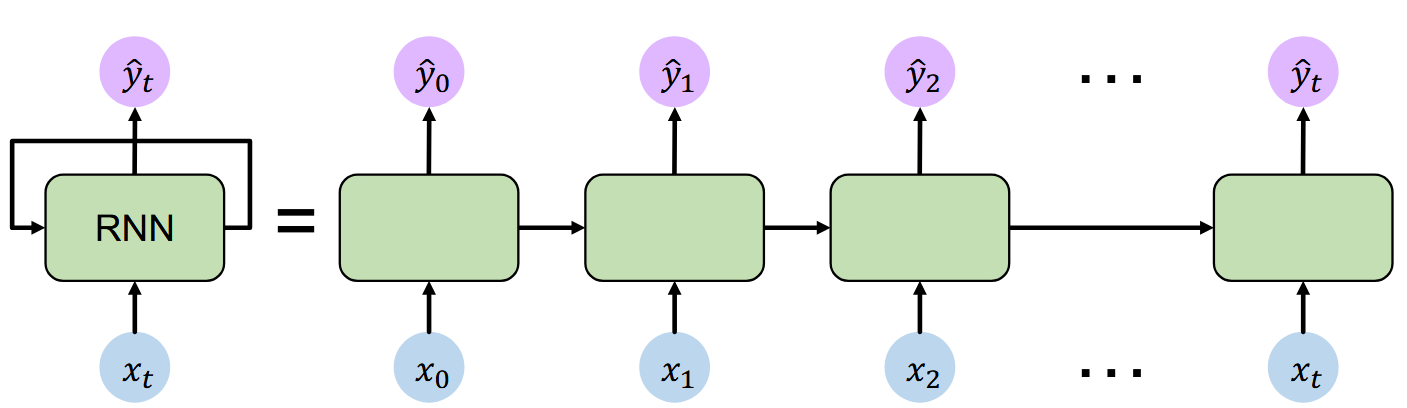
\includegraphics[width=10cm]{./figures/Model/RNN.png}
    \caption{RNN structure \fixme{cite3}}
    \label{fig:RNN}
\end{figure}

\hyperref[fig:RNN]{Figure 3} shows the unrolled flow of the RNN, where the arrows between each
block represents the passing of $h_t$, from one input to the next. The point
of the recurrence state $h_t$, is to show how the output of the model depends
on context from previous inputs plus $h_t$. This is especially relevant in our case, as
described in \hyperref[sec:gyroint]{section 3.1.1}, the accumulation of 
gyroscopic errors comes from the integration of the angular rate. As these
errors accumulate, the current error depends on the history of the gyroscope 
measurements. 

There are many problems with RNNs however, the biggest being the problem of exploding/vanishing
gradients. RNNs are trained via backpropagation through time, which propagates gradients across
timesteps. For long sequences, computing the gradient with respect to $h_0$ involes many factors
of repeated multiplication of Jacobians across time. This can lead to many values of the computation
being greater than 1, which explodes gradients leading to unstable training.
In the case, where many values are less than 1, this causes vanishing gradients where learning long-range
dependencies becomes difficult. Additionally, as the hidden state $h_t$ is propagated sequentially through
time, when performing backpropagation, training cannot be parallelised over timesteps. This results in 
a high training times compared to convolutional models.

Updated versions of the RNN have been proposed to solve the problem of vanishing and exploding
gradients. These being Long Short Term Memory (LSTM) and Gated Recurrent Units (GRUs). These methods
exploit the use of a cell state that does not need to do perform repeated multiplication of Jacobians,
however they are still subject to long training times \fixme{cite} and the gradient problem is not fully 
solved but mitigated \fixme{cite, cite}.

\subsubsection{Convolutional Neural Networks (CNNs)}
The next type of model considered was the CNN, even though typically it is used in computer
vision tasks; it has seen wide use in research relating to drift reduction \fixme{cite, cite, cite}. 
This model is based on the idea of convolving input data with a learnable filter to extract local 
features in the input data. The filter can be thought of like a window that slides over the 
data, and each filter has a defined set of weights in which it multiplies with input data.
This convolution operation can be described by the equation below: 

\begin{equation}
  z_f[t] = b_f + \sum_{c=1}^{C_{in}} \sum_{k=0}^{K-1} w_{f,c}[k] x_c[t+k- \lfloor K/2 \rfloor]
\end{equation}
\label{eq:12}

\begin{equation}
  y_f[t] = \phi(z_f[t])
\end{equation}

where $y_f[t]$, is the output of filter f, $b_f$ is a bias, $C_{in}$ is the input channels 
(for our case $C_{in}$ would be 3 for $\omega_x, \omega_y, \omega_z$), $K$ is the 
kernel/filter width, $w_{f,c}$ is the weights of the filter for a specific channel, 
$x_c$ is the input data of that channel, and $\phi$ is an arbitrary non-linear activation
function (typically ReLU).

For example if $K = 3$, the convolution will occur 
of the timesteps $x[t-1], x[t], x[t+1]$, this is how the convolution extracts local features 
in the input data.
 
Typically, these CNNs are made up of layers, where in each layer the number of filters 
grow e.g. $L1 = 16, L2 = 32, L3 = 64$ etc. These additional filters in later layers allow the
model to learn more complex feature sets based on the previous layers' filter. Zeiler et al.
\fixme{cite} shows this in their figure 2 where their convolutional network is used for image
classification.

\begin{figure}[H]
    \centering
    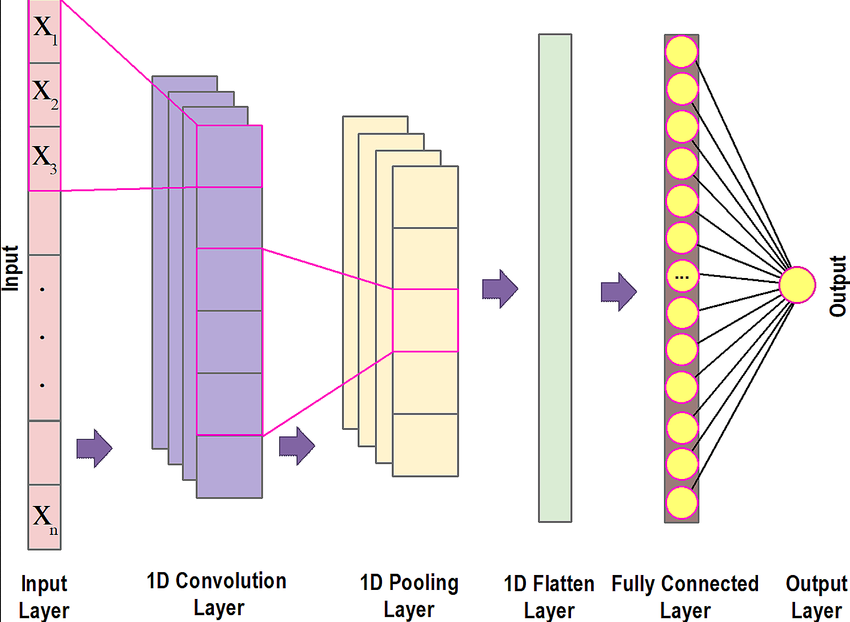
\includegraphics[width=10cm]{./figures/Model/CNN.png}
    \caption{1D CNN structure \fixme{cite}}
    \label{fig:CNN}
\end{figure}


CNNs are more attractive than RNNs due to its ability to be efficiently
trained by using parallelisation\fixme{cite}. As stated before, RNNs cannot exploit 
this, but CNNs can. This leads to the ability to test multiple different
iterations of a model where parameters and loss functions may be changed
to explore what effects they may have \fixme{see section}. CNNs also do
not suffer from vanishing//exploding gradients and are seen to be more
stable during training\fixme{cite}. 

However, unlike RNNs, baseline CNNs cannot produce outputs due to significant 
temporal information. It can extract local features and in 1D convolutions
it has some ability to traverse backwards through time but not to any
significant degree. As seen in \hyperref[sec:gyroint]{section 3.1.1}, 
the accumulation of drift is due to the integration of the angular rate
as we move forward in time. 

\subsubsection{Temporal Convolutional Networks (TCNs)}
TCNs are an extension of the baseline CNN and include two main differences
in their implementation as shown by Bai et al.\fixme{cite}. These differences
are the use of dilations that grow the receptive field allowing the network
to look back further in time and learn long-term information. Furthermore,
causal convolutions meaning, that the convolution operation cannot
look forward in time. To explain causality we can look back at  
\hyperref[eq:12]{equation 12} and modify this so 

\begin{equation}
  z_f[t] = b_f + \sum_{c=1}^{C_{in}} \sum_{k=0}^{K-1} w_{f,c}[k] x_c[t-k]
\end{equation}

\begin{equation}
  y_f[t] = \phi(z_f[t])
\end{equation}

The difference is that the $k$ is subtracted from $x[t]$. The causality
is enforced here as at time $t$, we cannot access future information unless
the model is to be used after data collection and not in a real time 
setting.

Dilations allow the model to look further back in time without the need
of increasing parameters for the same $K$ and $C_{in}$ used in convolutions. This is best represented in
the figure 5.

\begin{figure}[H]
    \centering
    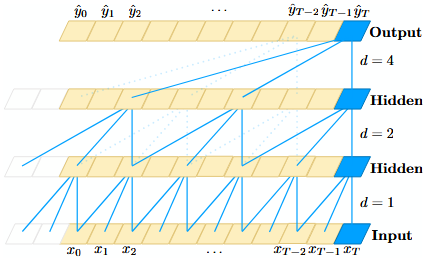
\includegraphics[width=10cm]{./figures/Model/dilations.png}
    \caption{CNN structure with dilations \fixme{cite}}
    \label{fig:dilations}
\end{figure}

As we can see in the diagram, as the dilations increase layer by layer
the output to the next layer looks further back into the history of
$x[t]$. This can be modelled by the equation

\begin{equation}
  z_f[t] = b_f + \sum_{c=1}^{C_{in}} \sum_{k=0}^{K-1} w_{f,c}[k] x_c[t-dk]
\end{equation}

where $d$ is the dilation factor of the layer. 


\subsubsection{Summary and Choice}
In summary, the choice has been to select the TCN. This is because it 
has the ability to look back in history and model long-term dependencies
between data, something baseline CNN cannot do. Additionally, like a CNN
it is quicker and more stable in training unlike an RNN. However, the TCN
does have its problems, these being extra data storage during its operation
and domain transfer. Unlike RNNs which only have store $h(t)$, TCNs needs
to take in a raw sequence upto its effective history length \fixme{cite}.
Domain transfer refers to transferring a model that has been trained in 
one domain (i.e. small receptive field) and applied to another domain
(i.e. large receptive field), where the TCN may perform poorly due to 
this change in domain.


\subsection{TCN Design and Parameters}
\subsection{Learning}


\newpage
\section{Loss Function Design}

\input{sections/Optimisation/optimisation}

\newpage

\section{Results}

\subsection{Evaluation Metrics}
Multiple metrics are used to evaluate the model performance, here in this section we outline each metric and give a motivation as to why. Throughout the results and evaluation both metrics are
reported together. The reason as to why both metrics are reported is that even though the geodesic angle error might decrease the yaw error may increase.

\subsubsection{Geodesic Angle Error}
To determine the error between the two quaternions that exist as rotations on SO(3), we use the geodesic rotation angle between the two
quaternions. This metric measures the minimal rotation needed to align the two quaternions.

\begin{equation}
    \epsilon_{\text{geo}} = 2\arccos\!\bigl(|\hat{q} \cdot q_{\text{gt}}|\bigr)
\end{equation}

The reason as to why we use the geodesic angle error is that it is the correct distance between two quaternions on SO(3). A Euclidean difference is not rotation invariant meaning 
$q$ and $-q$ would represent different rotations, where they are the same rotation on SO(3). It also captures the total orientation error (roll, pitch, and yaw) between the predicted orientation
and the ground truth.

\subsubsection{Absolute Yaw Error}
The equations below show how to calculate the absolute yaw error (AYE).

\begin{equation}
    \psi = \arctan2\!\bigl(2(wz + xy),\; 1 - 2(y^2 + z^2)\bigr)
\end{equation}

\begin{equation}
    \epsilon_{\text{yaw}} =
    \begin{cases}
        |\psi_{\text{pred}} - \psi_{\text{gt}}| & \text{if } |\psi_{\text{pred}} - \psi_{\text{gt}}| \leq 180^{\circ} \\
        360^{\circ} - |\psi_{\text{pred}} - \psi_{\text{gt}}| & \text{otherwise}
    \end{cases}
\end{equation}

The yaw is extracted from the quaternion rotation before the use of the equation above. Further, the AYE is wrapped over [0, 180], such that errors near $\pm180^{\circ}$ are not artificially inflated.

The reason as to why the AYE is an interesting metric to track is because of \fixme{mag section}. In this section it is mentioned that only the magnetometer can provide
a heading reference and thus with corrupted magnetometer measurements this drift in yaw becomes unbounded. By specifically looking at AYE, we can see how much the proposed solution is
able to correct yaw especially due to the test set conditions in \fixme{train/test/val section}. 

\subsection{Test Pipeline}

There a two different pipelines tested within this project. First, is dead reckoning (gyroscope integration only), this pipeline tests how the TCN performs by only providing $\omega$ corrections
which is applied additively to the raw gyroscope measurement. This test shows how the TCN performs solely as a gyroscope corrector. Second, is the full proposed solution with the integration of 
the MUKF. This tests shows the performance of the corrected gyroscope measurement in tandem with corrections applied from the accelerometer and magnetometer by the update step in the MUKF.

The rest of the results section will cover these two pipelines and report the per file statistics and the total aggregated statistics over the entire test set. 

\newpage
\clearpage
\section{Evaluation}
Looking at \fixme{table}, we can see that the deep-learning model produced significant improvements across all metrics in the 
entire test set. Both TCN Gyro and TCN + MUKF saw around a $38\%$ improvement in mean geodesic error and $40\%$ mean improvement in AYE, when compared to their raw 
gyroscope measurement counterparts. These metrics directly support the fact that the TCN model is able to address drift in tilt and heading
whilst both accelerometer and especially magnetometer 
are disturbed, which are the typical failure modes seen in orientation estimation with IMUs.

Furthermore, comparing TCN dead reckoning to raw gyroscope + MUKF, we can see that the TCN performs better, which highlights that 
the TCN alone does beat uncorrected raw gyroscope measurments even with corrections from an accelerometer and magnetometer. The comparison between
the two produces significant results with improvements in mean geodesic error  $14.6\%$, $31.6\%$ in  mean AYE, and $35.9\%$ in median AYE. This result
is expected as the test set does contain disturbed accelerometer and magnetometer conditions. 

Moreover, median improvements in TCN only of $44\%$ in geodesic error and $53\%$ in AYE, and $39.4\%$, and  $41.9\%$ in TCN + MUKF respectively, show 
a promising result that not only does the TCN produce fewer errors (mean) but also a more consistent output as well. Coupled with the P90 improvements of 
$41.2\%$ in geodesic error, and $44.1\%$ in AYE, for the TCN + MUKF, these results show that the entire distrubution landscape of errors is tighter. 
It shows that not only do we have overall better orientation estimates, but these improvements are more consistent and tail errors are supressed. 


\subsection{Trial 9: Undisturbed, Fast Rotation}
Looking at \fixme{table}, we can see that overall there have been significant improvements in all geodesic error metrics across the two pipelines, with the 
TCN + MUKF pipeline performing the best with an improvement of $37.2\%$ in mean geodesic error and the largest improvements in P90 and standard deviation of $54.8\%$.
This means that the model is able to provide meaningful corrections and that it is robust to tail errors. However, in the TCN Gyro pipeline we can see that
AYE actually gets worse ($-17.7\%$). 


\subsection{Trial 25: Disturbed Tapping}

\subsection{Trial 31: Disturbed Stationary Magnet}

\subsection{Trial 34: Disturbed Magnet attached 3cm}

\subsection{Trial 39: Disturbed, Mixed Conditions}

\subsection{Limitations of the Proposed Solution}

\subsection{Summary}

\newpage
\section{Conclusion and Next Steps}

\subsection{Semester 2 Aims}
With an understanding of all IMU operations, a baseline of how the UKF is able to fuse
sensor measurements and its performance, and with the residual block of the TCN implemented,
semester two is on track for the completion of this project. The main core of the model is the 
residual block and from here the rest of the work is covered in the next subsections.

\subsubsection{Model Hyperparameters}
The main thing to do is to determine multiple of the model hyperparameters such as, the filter
size, recpetive field, dilation factor, and the number of channels per residual block. For 
dilation factor, it is a common method to follow is $d = 2^i$ or $d = 4^i$ where $i$, 
is the layer number as seen by \cite{brossard_2020_denoising}. This is because by increasing
the dilation factor the model can see further back in time and use this information to more
accurately predict the accumulation of errors. However, as this is not a standard rule a wide
variety of dilation factors will be used to test model performance. 




\subsubsection{Model Training}


\subsection{Summary of Progress}
During Semester One, the project progressed from initial understanding 
of the challenges faced in orientation estimation, to exploration and 
designing of deep learning models. Much of the work conducted
had been research using academic literature and online
lectures. With foundational knowledge gained in all areas of the project,
it has ensured that Semester Two can be focused on the completion    
deep learning model to address the questions posed in
\hyperref[sec:question]{section 1.3}. Furthermore, the exploration of how the 
baseline UKF performed also gave me vital understanding in how the model should attempt
to learn gyroscopic drift.

\subsection{Challenges}
The primary challenge encountered during this semester stemmed from having
no prior knowledge of IMU operations and deep learning. This led to 
extensive research needed for the completion of the project, 
which slowed down the implementation of the model. However, now having
concluded research I have been able to make informed decisions behind 
the selection of model, optimisation through normalisatio, and measurements
that accurately assess the performance of the model. 

\subsection{Skills Developed}
The main skill developed has been learning how to assess and evaluate 
literature and ascertain the correct conclusions to be able to be applied
to this project. My ability to use the PyTorch library and 
Python skills have developed to a significant degree in which modelling,
measurements, and analysis will be conducted within Python. In addition, 
my technical writing capabilities have also progressed especially compared
to my third-year project. 


\newpage
\printbibliography



\end{document}
